\chapter{Related Work}
\label{cha:related-work}
In the following chapter, the inspiration and foundation for this project are presented. Firstly, literature about similar projects is outlined, followed by an introduction to the main technologies examined, and finally a short rundown of the technologies used for experimentation and evaluation is given. 

\section{Literature}
Multiple authors have already evaluated \ac{DASH} video streaming both in relation to other protocols, as seen in \citet{aloman2015performance}, but also in a \ac{P2P} network as done by \citet{gazdar2017toward}. In terms of performance of \ac{P2P} networks, \citet{nguyen2009p2p} have evaluated video acquisition with a \ac{DHT} network and \citet{qiu2004modeling} have done a theoretical approach while also listing important aspects to consider when building a \ac{P2P} network. Since the focus of this thesis is on video viewing performance it is also important to consider how videos are watched, which \citet{broxton2013catching} have done by defining a socialness factor to videos, based on how viral they are, which affects how a video is watched over time in a \ac{P2P} network.
\\


\citet{aloman2015performance} have evaluated \ac{DASH} (which will be explained in detail in \autoref{sec:rel-dash}) and two other streaming protocols (\ac{RTSP} and \ac{RTMP}) for on-demand and live video streaming in both 4G and WiFi conditions. Evaluation is done in terms of \ac{QOE} metrics with a large amount of parameters including: Resolution, bitrate, framerate, interval between \acsp{I-frame}, packet loss rate and delay. \ac{QOE} was estimated through the quality of service with an algorithmic model, rather than user based scores.

In terms of results, when introducing packet loss and delays \ac{DASH} sacrifices throughput in order to maintain good \ac{QOE} whereas the other protocols resort to re-buffering. \ac{DASH} does however have larger initial buffering time, when starting the video, and as packet loss and delay increases more time is required to fill the buffer initially. They conclude that \ac{RTSP} is more efficient for starting the video initially but at the expense of packet loss in the video stream played. They claim this is due to \ac{RTSP} being a \ac{UDP} based protocol where \ac{DASH} is \ac{TCP}. They claim the extra time buffering is worth it as re-buffering events are almost entirely eliminated. In their results, \ac{QOE} (measured in \ac{MOS}) is noticeably higher when using \ac{DASH} in the same scenarios. In their testing, packet loss affected \ac{QOE} more than delay.
\\


\citet{gazdar2017toward} have built a streaming system based on the \ac{P2P} protocol BitTorrent instead of \ac{IPFS}, while also using \ac{DASH} as the video player. To accomplish this they needed to make small adjustments to the video's \ac{MPD} metadata file by adding information about the tracker. This way the \ac{MPD} file alone is enough to start the video streaming process.

For tests in the system they focused on segment missing rate and \ac{UX}, with a variety of quantity of peers, start delay and cache sizes. They observed that the system's performance decreased as the network grew larger, by having more missed segments and more waiting time on playback. The \ac{UX} also suffered most when viewing at a high quality. These conclusions contradict our hypotheses that a large network should help increase the availability and thereby a client's \ac{UX}, but this might be due to BitTorrent not being suitable for this purpose, or that their peer selection algorithm is lacking which they themselves point out might be the case.
\\


\citet{nguyen2009p2p} argue that 60\% of the commonly used bandwidth cost can be saved using a \ac{P2P} system as opposed to a client-server model. The \ac{P2P} system uses the \ac{DHT} chord as its network architecture, and the video files are broken into multiple smaller pieces which are then dispersed across peers in the network with redundant copies. To ensure that files are not lost as peers leave and join the network, the new peers share the burden of storing files of the rare pieces, so that it is always possible to reconstruct the video. When streaming a video the system prefers pieces from different peers as this creates multiple internet routes, resulting in increased bitrate. In their testing they store the packets in two ways and compared these. The first is to distribute the packets as is (non-\ac{NC}) and the other is having the packets be random linear combinations of the original packets (\ac{RNC}). The results focused on the probability of being able to retrieve a piece and the latency to do so, and the \ac{RNC} scheme performed best in both cases.
\\


\citet{qiu2004modeling} perform a theoretical evaluation of a BitTorrent network, and list four issues that have to be addressed to understand the system.

\emph{Peer evolution} is how many peers are in the network and how they act in terms of arrival, departure and bandwidth.

\emph{Scalability} is how the system's performance should increase as the number of peers grows, which also state that network performance can be measured by average file downloading time.

\emph{File sharing efficiency} is how the system must be designed such that peers are connected to peers that have the wanted file, and the bandwidth of each peer must be fully utilized.

Finally, the system needs \emph{incentives to prevent free riding}, meaning one should not be able to download files without contributing to the network.

Based on these issues a flow model of a BitTorrent network was constructed, from which they could infer averages of parameters such as seeds, downloaders and download time as functions of arrival rate. It's also shown that BitTorrent had incentives to prevent free riding and a Nash equilibrium existed, meaning it would be optimal for the peers to upload at their maximum speed.
\\


\citet{broxton2013catching} have analyzed the characteristics of viral videos on YouTube in terms of how such are viewed in respect to a socialness level defined in the article. To qualify as a social video, it has to be viewed through sharing, meaning that access to the video is done through an external link, instead of pasting the URL directly. An unsocial video is instead found through a search or some discovery mechanism within the site itself. The socialness level can then be defined by how many of the videos views come from social sources versus nonsocial. The socialness of a video also evolves over time and the percentage of social views drop over time, e.g. if the video is shared more when it is new. It is noted that highly shared videos tend to generate more views than less shared videos. It is also stated that the socialness of a video varies depending on the genre of the video. The behaviour of social views also depend on the source, social views generated through the website \textit{Twitter} drop off harder and peak more in views compared to social views generated through a social network like \textit{Facebook}.


\section{Frameworks and Technologies}
\label{sec:fram-techn}
In this section frameworks and technologies relevant to or crucial for the project are presented.

\subsection{\acl{IPFS}}
The \ac{IPFS} is a \ac{P2P} distributed file system, as specified in \citet{benet2014ipfs} and implemented by Protocol Labs\footnote{\url{https://ipfs.io/}}.

It consists of several different properties of successful \ac{P2P} systems such as \ac{DHT}, BitTorrent, Git and \ac{SFS}. The \ac{IPFS} protocol constructed consists of the following sub-protocols, among others.

\subsubsection{Identity}
All nodes are identified by a public key of a SHA-256 cryptographic hash. To instantiate a new identity, the node must solve a static crypto puzzle as utilized in S/Kademlia\cite{baumgart2007skademlia}.

\subsubsection{Routing}
The routing system is capable of finding other peers' addresses in the network and determine which peers serves a wanted object. Using a \ac{DSHT} based on S/Kademlia and Coral \cite{baumgart2007skademlia, freedman2004coral}. A distinction of object's size and usage patterns determines where values are stored. If they are less than 1KB they are stored directly on the \ac{DHT}, otherwise a reference of the identity of peers serving the block is stored instead. 


\begin{table}[ht]
\myfloatalign
\caption{\acs{IPFS} Overview.}
\label{tab:ipfs_overview}
%\begin{tabularx}{\textwidth}{l|r|r|r}\toprule
\begin{tabularx}{\textwidth}{cccc}\toprule
\tableheadline{Role} & \tableheadline{Layers} & \tableheadline{Instances} & \tableheadline{Inspiration} \\\midrule
Using the data                      & applications  & dash.js   & web           \\\midrule
\multirow{2}{*}{Defining the data}  & naming        & \acs{IPNS}      & \acs{SFS}     \\
                                    & merkle-dag    & \acs{IPLD}\footnotemark      & git           \\\midrule
\multirow{3}{*}{Moving the data}    & exchange      & |         & BitTorrent    \\
                                    & routing       & libp2p\footnotemark    & \acs{DHT}     \\
                                    & network       & |         & --            \\
\bottomrule
\end{tabularx}
\source{\url{https://youtu.be/HUVmypx9HGI?t=33m12s}}
\end{table}
\footnotetext[2]{\url{https://ipld.io/}}
\footnotetext{\url{https://libp2p.io/}}


\subsubsection{Exchange}
Distribution of data happens by exchanging blocks with a protocol called BitSwap, which is inspired by the way BitTorrent exchanges blocks of data. Each peer has a list of blocks they want and a list of what they already have, similar to BitTorrent but instead it is for the entire network.

In BitSwap values are given to each block, meaning to get something from another peer something usually has to be given in exchange. If a peer has little or nothing from the other peer's wantlist it prioritizes blocks wanted by the other over blocks from its own wantlist. This helps reduce the amount of rare blocks in the network.

The protocol also incentivises seeding even when the peer does not currently need any blocks. The idea is that this debt will be repaid in the future, and as such each peer tracks how much they owe, and send more blocks to their debtors. The debt is also used as a measure of trusts, which protects against malicious users.

Nodes also keep ledgers accounting transfers with the other nodes, to track history. When a connection is established Ledger information is exchanged, if it does not match exactly the ledger is recreated from scratch and all accrued trust and debt is reset. The authors claim that malicious users can purposefully lose their debt but this should not be worth the loss in trust.

\begin{figure}[ht]
    \centering
    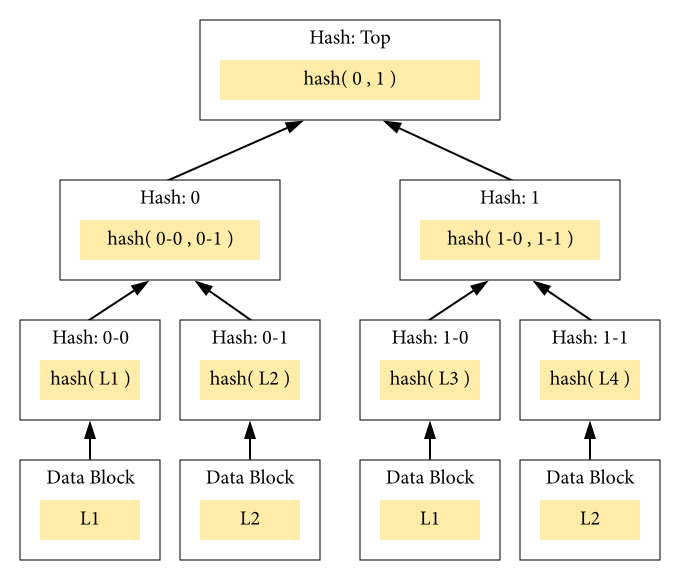
\includegraphics[width=\textwidth]{merkle}
    \caption[A Merkle Tree]{An example of a binary Merkle tree, conceptually like Merkle-\acsp{DAG}. Hashes 0-0 and 0-1 are the hash values of data blocks L1 and L2, respectively, and hash 0 is the hash of the concatenation of hashes 0-0 and 0-1.}
    \label{fig:merkle_tree}
    \source{Adaption of \url{https://commons.wikimedia.org/wiki/File:Hash_Tree.svg}}
\end{figure}

\subsubsection{Objects}
\label{sec:ipfs-objects}
The individual blocks are linked together using Merkle \acp{DAG}, which is a directed acyclic graph where each node has a cryptographic hash, and the hash of the parent verifies the children (See \autoref{fig:merkle_tree}). This structure is a generalization of the git data structure and provides: addressing of content using the hashes, tamper resistance since it can be detected and de-duplication as data that holds the same content will also hash to the same thereby only needing to be stored once. From the hash addresses files can also be traversed with a traditional UNIX file system path if the hash is that of a folder.
Since hashes are used to address files, newer versions of a file will hash differently, which means that tracking these is done using additional versioning.



\subsection{\acl{DASH}}
\label{sec:rel-dash}

\begin{figure}
    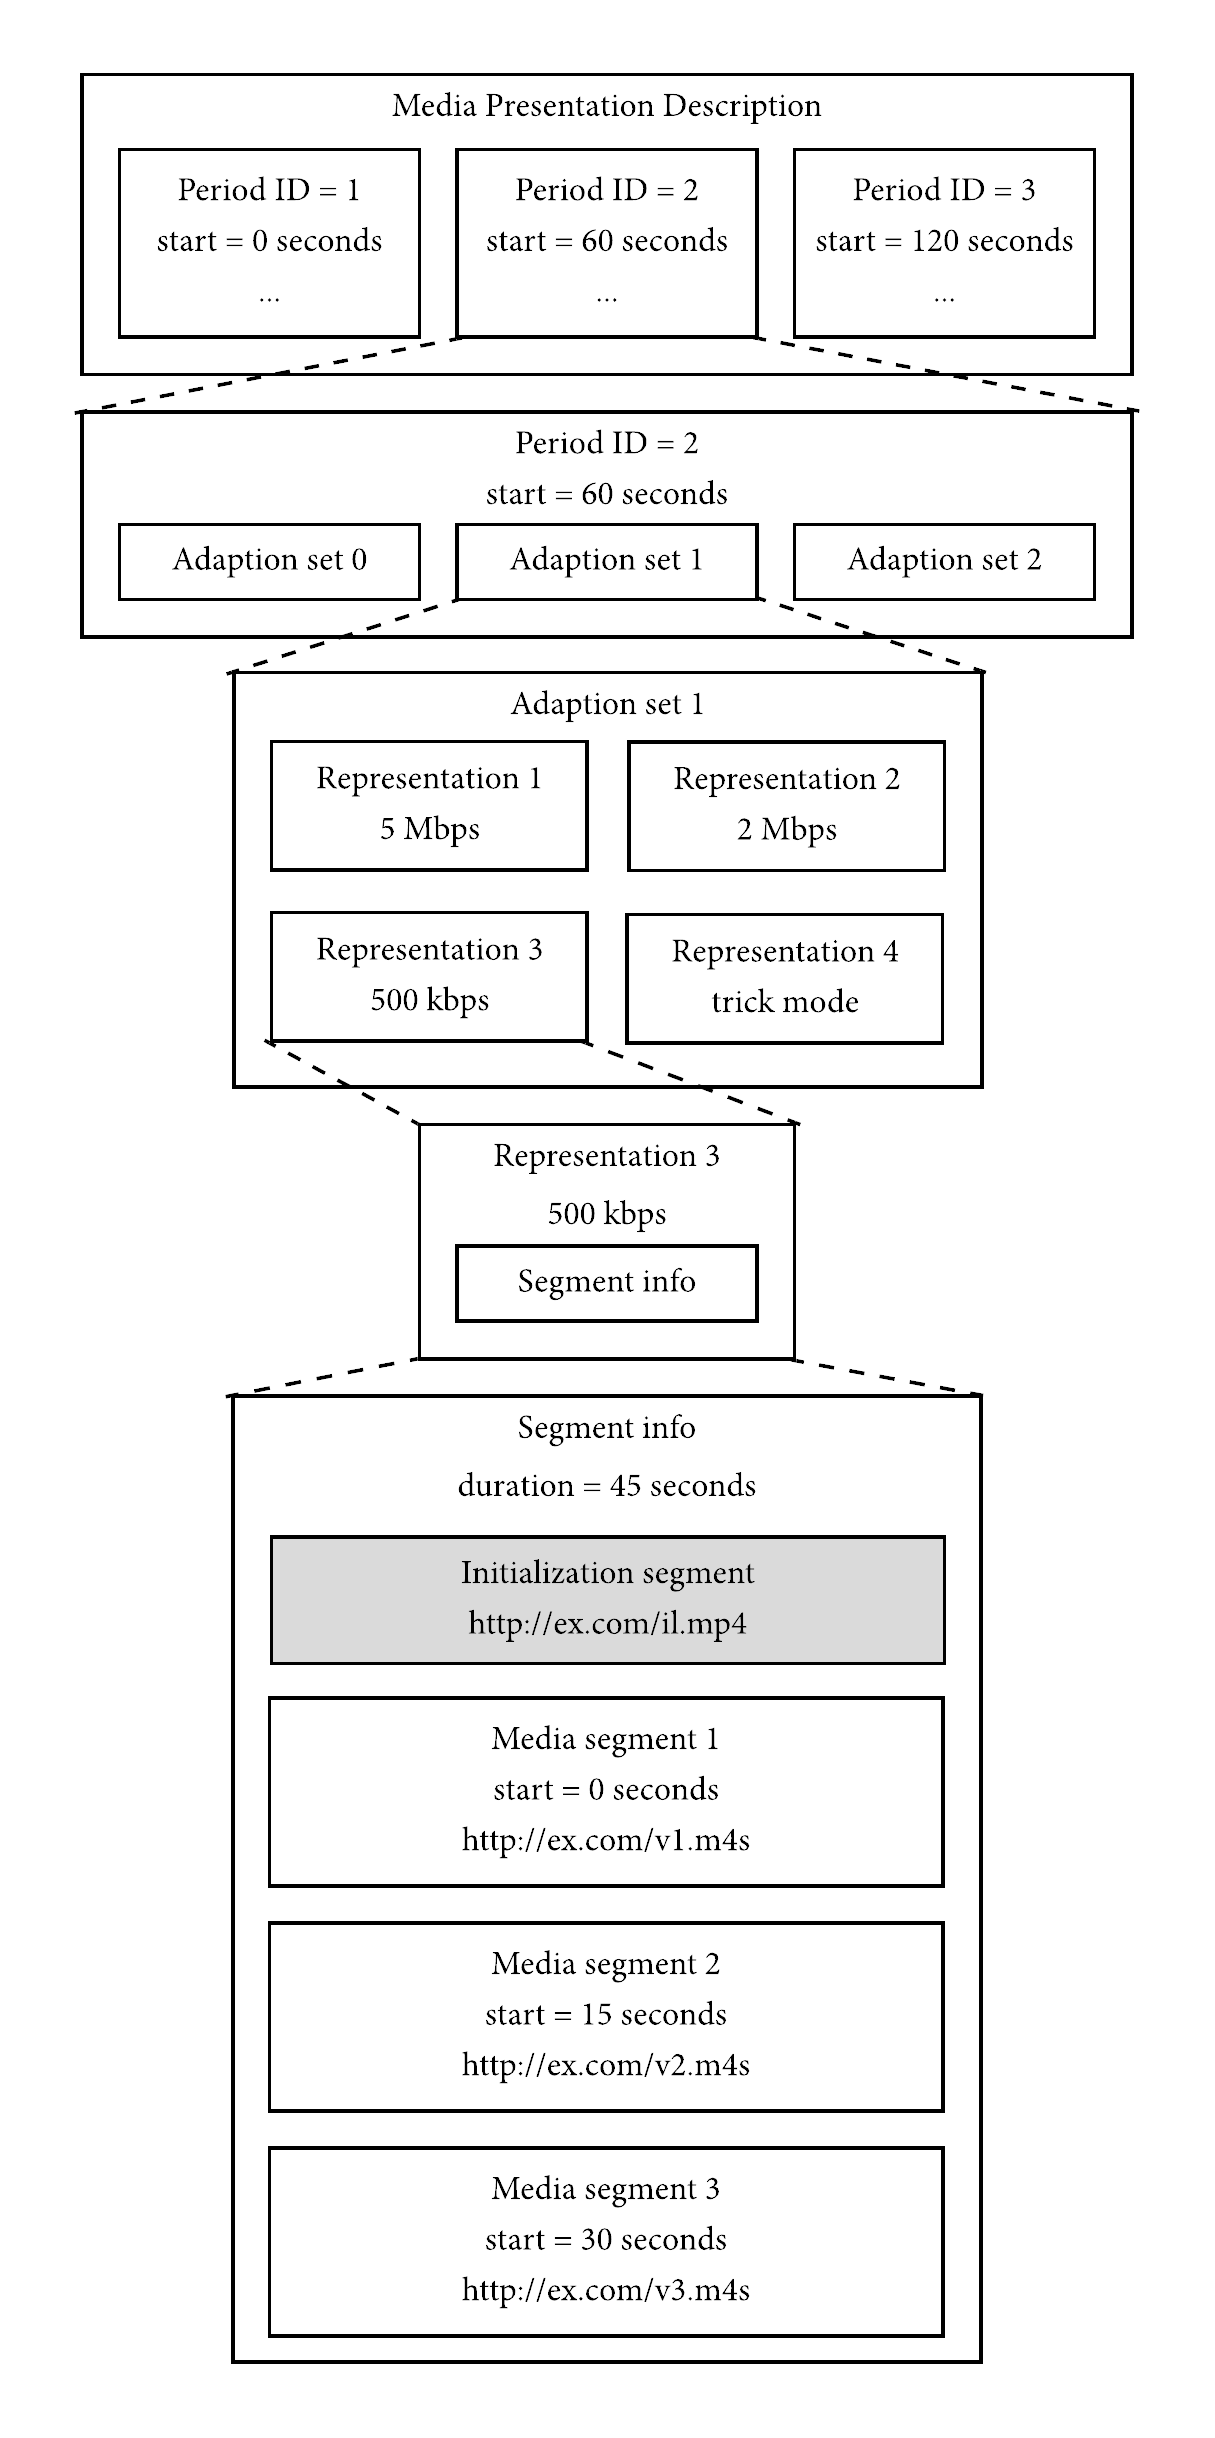
\includegraphics[width=\textwidth]{mpd}
    \caption[The structure of an \acs{MPD}.]{The structure of an \acs{MPD}.}
    \label{fig:mpd_structure}
    \source{Adaption of citet[Figure 3 on p. 65]{sodagar2011mpeg}}
\end{figure}

\ac{DASH} is an adaptive bitrate streaming technique that enables high quality streaming over \ac{HTTP}. This is done by breaking the content into smaller file segments, each containing a short playback interval. The standard defines that each of these segments can be served at different bitrates, allowing the \ac{DASH}-client to choose the next segment to download, based on its current network conditions.
This makes it possible to serve a stream that adapts seamlessly to deliver streams with high quality and few stalls and re-bufferings, based on the changing conditions of the network.

The segments are described by an \ac{MPD} file, in which information about the files, such as timing, \acp{URL}, bitrates and resolution resides. From the \ac{MPD} the multimedia selection can then be made based on user preferences (such as specific language audio streams), device capabilities (such as hardware decoding) and the previous mentioned conditions of the network.

The \ac{DASH} Industry Forum (DASH-IF), consisting of Netflix, Google and Microsoft among others, helps push to implementation of the specification\cite{ISO23009}. This is done by creating guidelines for usage and libraries such as \texttt{dash.js}\footnote{\url{https://github.com/Dash-Industry-Forum/dash.js}} that adds \ac{DASH} compatibility in a \ac{HTML} video player using JavaScript.

\section{Testing Framework}
In this section the technologies used to create the testing framework are presented.

\subsection{Docker}
 Docker\footnote{\url{https://docs.docker.com/}} is a tool that can package an application and its dependencies in a virtual \emph{container} that can run on any Linux server. In contrast to \acp{VM}, containers share \ac{OS} and bins/libraries where appropriate, while still being isolated (See \autoref{fig:vm_vs_container}). This results in lower overhead for each instance running, making it possible to easily scale and run more instances on the infrastructure (See \autoref{fig:vm_vs_container}).
 
 \begin{figure}[ht]
    \myfloatalign
    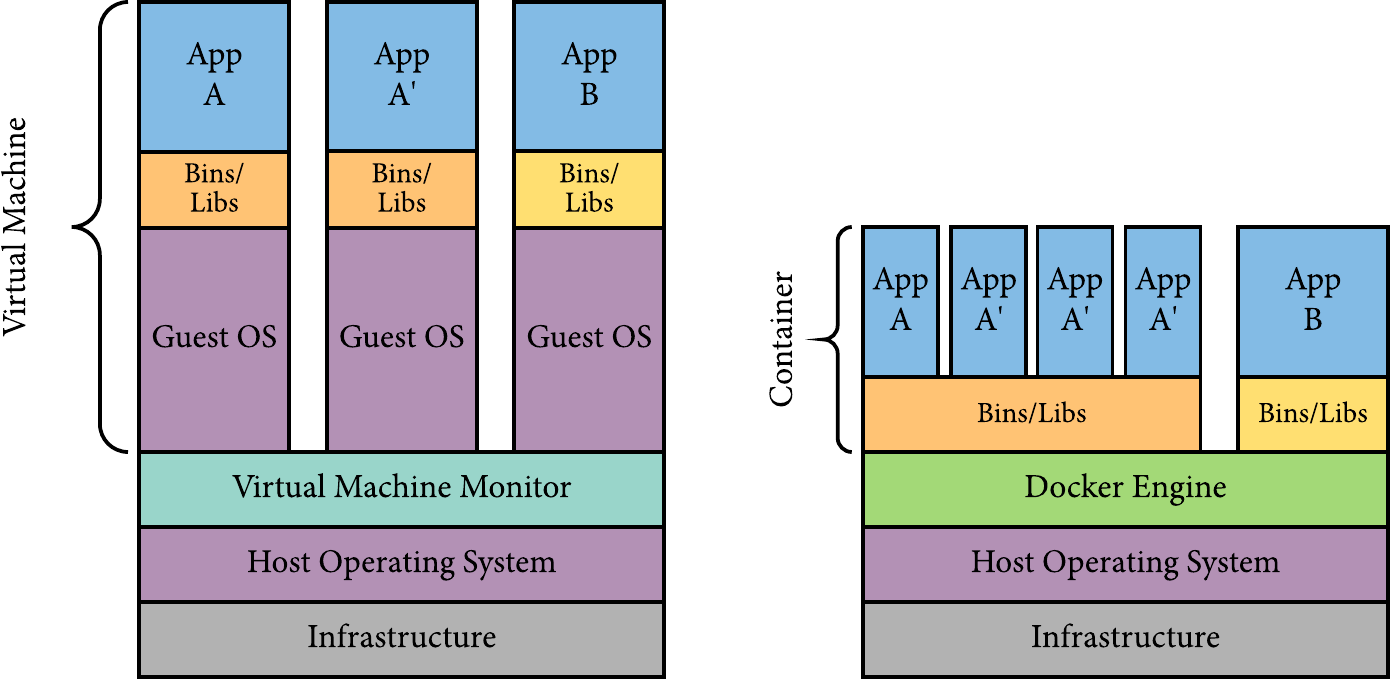
\includegraphics[width=\textwidth]{vm.png}
    \caption[Comparison of \acs{VM} and Docker]{Comparison of the overhead present in virtualization done by a \acl{VM} and by Docker}
    \label{fig:vm_vs_container}
\end{figure}
 
 Individual user spaces are also provided to the containers, meaning that it looks like a real computer, from the point of view of the applications running inside.
The shared kernel results in less overhead per container when compared to other virtualization approaches, but is less flexible since it cannot host an \ac{OS} different from the host machines. Due to the low resource cost of containers, Docker promotes an application-centric container model\cite{merkel2014docker}, so only individual applications or services are run inside, resulting in a loose coupling of the components in the system, as seen with microservices. 
By running programs in containers hardware independence is achieved due to the abstraction layer of Docker, while also gaining easy access to CPU and memory management.

\subsubsection{Glossary}
\begin{itemize}
    \item \textit{Image:} 
    A Docker image is the basis for the container. It describes changes from a root filesystem and execution parameters to use within a container during runtime. An image can never change as it does not have a state.
    
    \item \textit{Container:}
    A Docker container is the runtime instance of the Docker image. It consists of an image, execution environment and a standard set of instructions.
    
    \item \textit{Entrypoint:}
    An entrypoint of a Docker image is the application to run, when the image is instantiated as a container.
    
    \item \textit{Compose:}
    Docker compose is a tool for defining and running multi-container application, within a single file and command to get it running. Allowing containers to be setup with dependencies of other containers, and to start them in the correct order.
    
    \item \textit{Virtual machine:}
    A \acl{VM} is a program that emulates a complete computer and its hardware, while sharing physical resources with the host computer. Compared to containers a \ac{VM} is heavier to run as it is more isolated and resource sharing is minimal.
    
    \item \textit{Volume:}
    A volume is a specially-designated directory within the containers or even on the host file system. Volumes are designed to persist data longer than the life cycle of the container using it.

\end{itemize}


\subsection{Chaos Engineering \& Pumba}
\label{sec:framework_pumba}
Chaos Engineering is the discipline of experimenting on a distributed system in order to build confidence in the system’s capability to withstand turbulent conditions in production\footnote{\url{http://principlesofchaos.org/}}.

The philosophy behind Chaos Engineering is that even though each part in a distributed system works correctly, systemic weaknesses can exist, and to discover these we emulate and manage chaos inherent in the system. This empirical, systems-based approach builds confidence in the ability of these systems to withstand real conditions, through observations of controlled experiments.

Chaos engineering is done by setting up an experiment to uncover systemic weakness.
First, a \emph{steady state} is defined by some measureable output, that indicates normal behaviour. The hypothesis is that the \emph{steady state} will continue throughout the experiment.
Secondly, variables that reflect real world events are introduced (eg. server crashes, low bandwidth, spike in traffic, etc.).
Thirdly, the hypothesis is tried disproved by examining the \emph{steady state} data.
The harder it is to disrupt a \emph{steady state}, the more confidence is gained in the behaviour of the system, and discovered weaknesses can be targeted for improvement, before the behaviour manifests system-wide.

Netflix developed this practice with their program Chaos Monkey which would randomly shut down services, and later expanded to a set of open sourced tools called Simian Army\footnote{\url{https://github.com/Netflix/SimianArmy}} built for different turbulent conditions, but targeted at \ac{VM}'s.

Pumba\footnote{\url{https://github.com/gaia-adm/pumba}} is a chaos testing tool for containers in Docker. It can manipulate processes, their performance and network.

\section{Summary of Related Works}
Multiple authors have already worked with \ac{DASH} video streaming and \ac{P2P} networks, with differing kinds of evaluation techniques and focus points.

\citet{aloman2015performance} evaluated \ac{DASH} compared to alternative streaming protocols, they evaluated based on on \ac{QOE} with varying bitrate, I-frame intervals and more. \citet{gazdar2017toward} built \ac{DASH} streaming on top of BitTorrent with small modifications to the \ac{MPD} file format. Their testing focused on segment missing rate and \ac{QOE} with varying network size, start delay and cache sizes. \citet{nguyen2009p2p} found that bandwidth in the network could be saved by using a \ac{DHT}. Their testing had files as segments either stored as is, or as a linear combinations of the originals, and they tested the likelihood and latency of getting file pieces. \citet{qiu2004modeling} identified issues a \ac{P2P} system had to handle, based on this they built a flow model for BitTorrent, where they argued that freeriding is discouraged. \citet{broxton2013catching} analyzed virality of YouTube videos, and defined socialness based on how these videos were shared. They found a correlation between socialness and how viewership evolved over time.

%%% Local Variables:
%%% mode: latex
%%% TeX-master: "../ClassicThesis"
%%% ispell-dictionary: "british" ***
%%% mode:flyspell ***
%%% mode:auto-fill ***
%%% fill-column: 78 ***
%%% End:
